\documentclass[12pt,a4paper]{scrartcl}
\usepackage{scrlayer-scrpage}
\pagestyle{scrheadings}
\ohead{Baumann Martin, 01527563}
\ihead{MLA Homework 3 Report}

\usepackage{lmodern}
\usepackage{float}
\usepackage{listings}

\usepackage{graphicx}
\usepackage{subfig}
\usepackage[T1]{fontenc}

\usepackage{epstopdf}
\usepackage{amsmath}
\usepackage{amssymb}
\usepackage{siunitx}
\sisetup{exponent-product = \cdot, output-product = \cdot}
\usepackage{prettyref}
\newrefformat{fig}{Figure \ref{#1}}
\newrefformat{tab}{Table \ref{#1}}
\newrefformat{eq}{(\ref{#1})}

\usepackage{multirow}
\newcommand{\matr}[1]{\mathbf{#1}}

\usepackage{physics}
\usepackage{tikz}

\begin{document}
	
	\section*{Problem 3.1}
	
	\subsection*{Surface plot}
	
	The error surface is shown in \prettyref{fig:ex3_1_err_surface}. 
	The loss is computed as the sum of the individual losses over all samples.
	\begin{equation}
		J\left(\matr{w}, \matr{x}^{(i)}, y^{(i)}\right) = \left(y^{(i)} - \matr{w}^T\matr{x}^{(i)} \right)^2 \label{eq:ex3_1_loss}
	\end{equation}
	
	This can be written as a quadratic form
	\begin{equation}
		\sum_{i=0}^{N-1} \matr{w}^T \matr{x}^{(i)} \left(\matr{x}^{(i)}\right)^T \matr{w} - 2y^{(i)} \matr{w}^T\matr{x}^{(i)} + \left(y^{(i)}\right)^2 = \matr{w}^T \matr{A}\matr{w} +\matr{b}^T\matr{w}+c.
	\end{equation}

	By evaluating 
	\begin{equation}
		\matr{A} = \sum_{i=0}^{N-1} \matr{x}^{(i)} \left(\matr{x}^{(i)}\right)^T = \begin{bmatrix}
			\num{120.4} & \num{6.25} \\ \num{6.25} & \num{100.1}
		\end{bmatrix}
	\end{equation}
	it can be seen that this matrix is positive definite and the loss is therefore convex in the argument $\matr{w}$.
	
	\begin{figure}[H]
		\centering	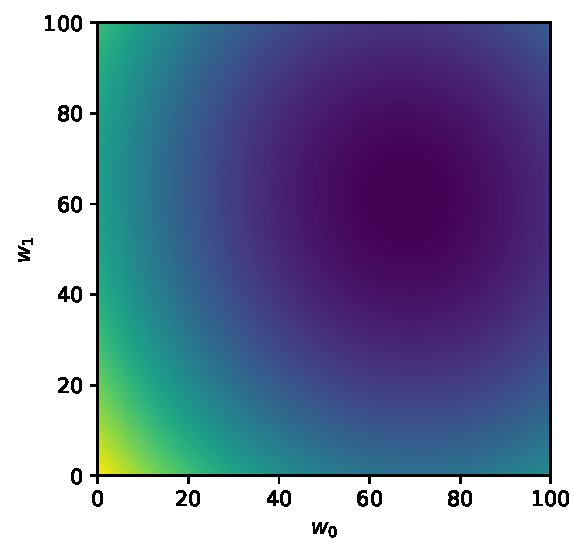
\includegraphics[width=0.65\linewidth]{figs/ex3_1_surf.pdf}
		\caption{Error surface}
		\label{fig:ex3_1_err_surface}
	\end{figure}
	
	\subsection*{Analytical gradient}
	
	The loss for a single sample by \prettyref{eq:ex3_1_loss}.
	
	The gradient with respect to the weight vector is therefore
	\begin{equation}
		\nabla_\matr{w} J\left(\matr{w}, \matr{x}^{(i)}, y^{(i)}\right) = 2\left(y^{(i)} - \matr{w}^T\matr{x}^{(i)} \right)\left(-\matr{x}^{(i)}\right) = 2\matr{x}^{(i)}\left(\matr{w}^T\matr{x}^{(i)} - y^{(i)}\right).
	\end{equation}
	
	\subsection*{Batch-Gradient-Descent}
	
	For the settings $K=200$, $\alpha = 10^{-2}$ and the initial weight $\matr{\hat{w}}^{(0)} = [1, 1]^T$ the history of the loss and a scatter plot of the weights are shown in \prettyref{fig:ex3_1_bgd}.
	The final weight vector is $\matr{\hat{w}}^{(K)} = [67.53, 60.17]^T$
	
	\begin{figure}[H]
		\centering	
		\subfloat[Scatter plot of weight vectors]{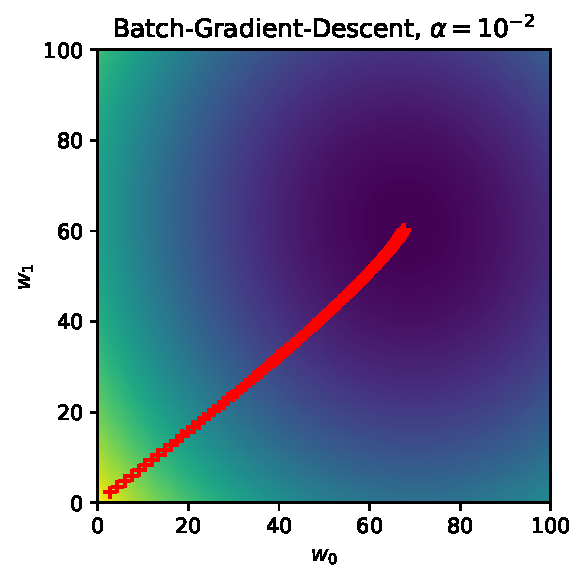
\includegraphics[width=0.5\linewidth]{figs/ex3_1_surf_bgd.pdf}}\\
		\subfloat[Loss]{	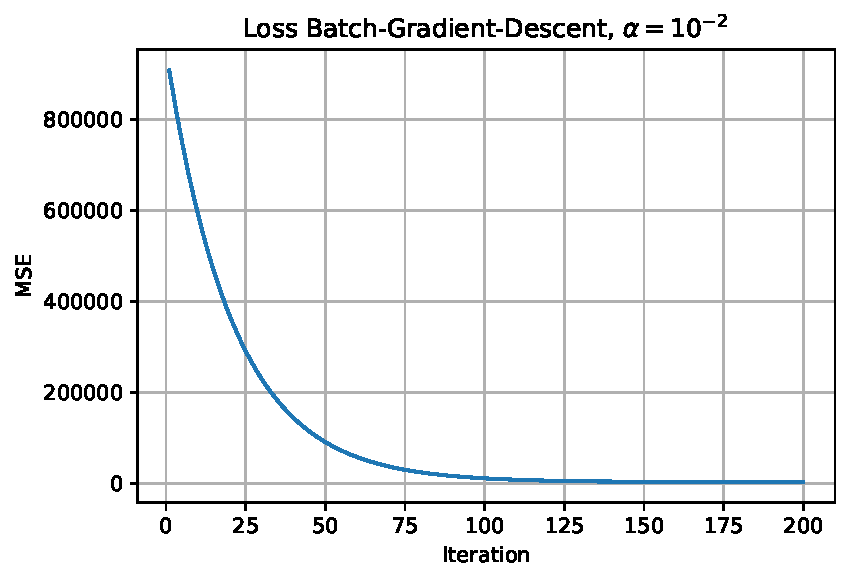
\includegraphics[width=0.6\linewidth]{figs/ex3_1_loss_bgd.pdf}}
		\caption{History of optimization with BGD}
		\label{fig:ex3_1_bgd}
	\end{figure}
	
	
	\subsection*{Stochastic-Gradient-Descent}
	
	For the settings $K=200$, $\alpha = 10^{-2}$ and the initial weight $\matr{\hat{w}}^{(0)} = [1, 1]^T$ the history of the loss and a scatter plot of the weights are shown in \prettyref{fig:ex3_1_sgd}. The final weight vector is $\matr{\hat{w}}^{(K)} = [67.54, 60.17]^T$.
	
	\begin{figure}[H]
		\centering	
		\subfloat[Scatter plot of weight vectors]{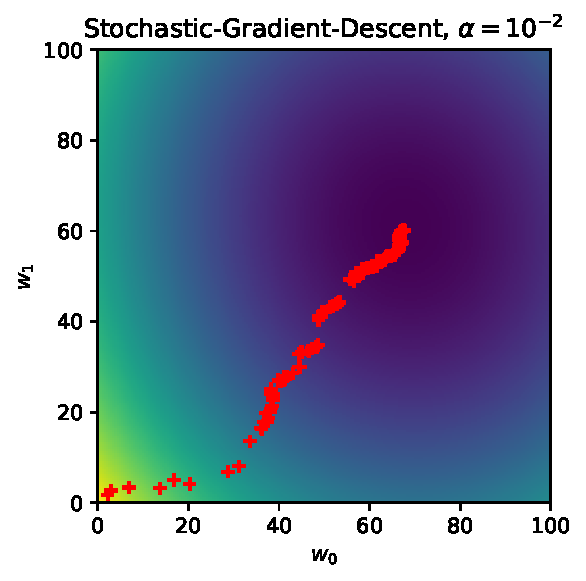
\includegraphics[width=0.5\linewidth]{figs/ex3_1_surf_sgd.pdf}}\\
		\subfloat[Loss]{	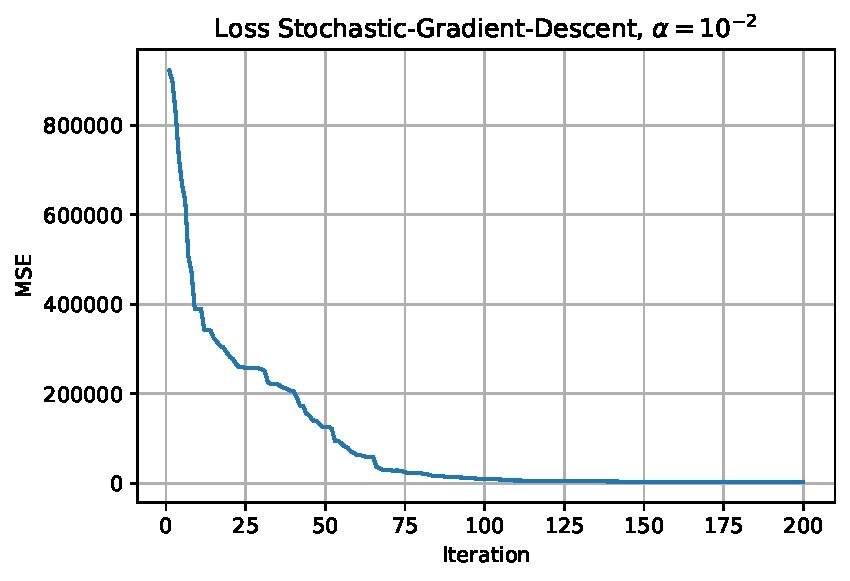
\includegraphics[width=0.6\linewidth]{figs/ex3_1_loss_sgd.pdf}}
		\caption{History of optimization with SGD}
		\label{fig:ex3_1_sgd}
	\end{figure}
	
	
	\subsection*{Discussion SGD and BGD}
	
	BGD almost approaches the optimum in a straight line as can be seen from the scatter plot. For SGD the trajectory of the weight vector is more noisy, but it still approaches the minimum of the loss.
	As SGD computes the gradient on a single sample, it is more noisy and therefore the direction of the gradient varies from iteration to iteration. For BGD the gradients of all samples are averaged and therefore less noisy which leads to a more steady path towards the optimum.
	
	The same behaviour can be seen in the loss plots, where the loss decreases strictly monotonic for BGD, whereas for SGD the loss sometimes decreases rapidly and then it stays almost constant for some iterations.	
	
	\subsection*{Effect of learning rate}
	
	In \prettyref{fig:ex3_1_learning_rate} the effect of the learning rate on both BGD and SGD is shown.
	Overall it can be seen, that the Loss decreases significantly faster with the higher learning rate. For BGD the trajectory of the weights is nearly unchanged, it just approaches the optimum faster. 
	For SGD the weights show a significantly larger fluctuation close to the optimum and from the loss curve it can be seen by the bumps close to 0, that sometimes the loss even increases from one iteration to another.
	
	For a learning rate of $\alpha = 1$ both solvers diverged, the loss increased and the weight vector does not approach the minimum of the loss.
	
	Overall a higher learning rate is beneficial because less iterations are needed to train the model, but it can't be set too high because this might lead to divergence or the weights walking around the optimum for a long time.
	
		\begin{figure}[H]
		\centering	
		\subfloat[Scatter plot of weight vectors for BGD]{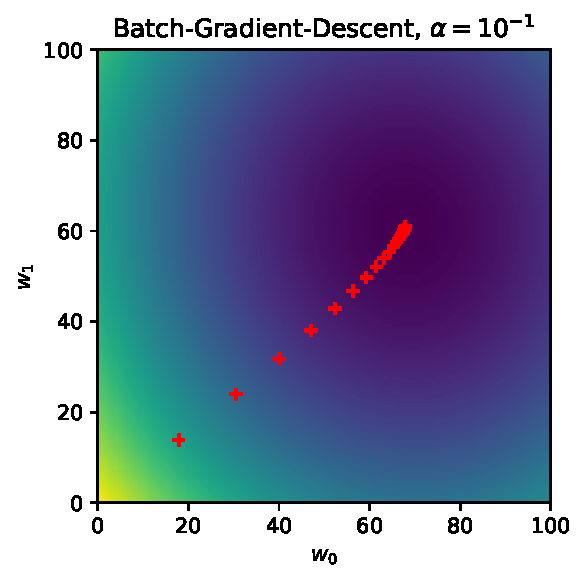
\includegraphics[width=0.5\linewidth]{figs/ex3_1_surf_bgd1.pdf}}
		\subfloat[Scatter plot of weight vectors for SGD]{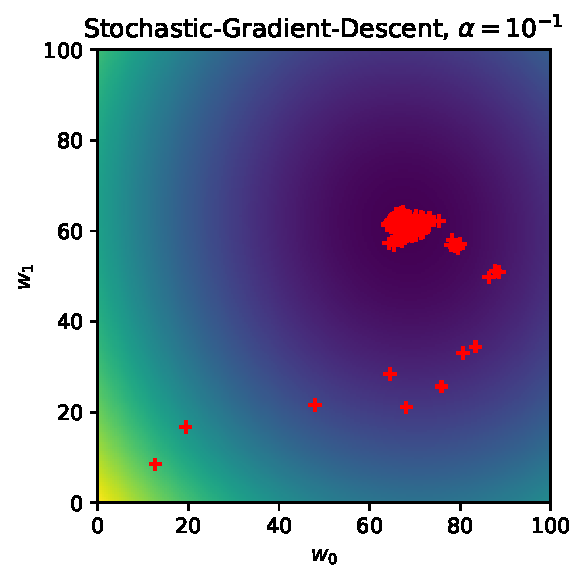
\includegraphics[width=0.5\linewidth]{figs/ex3_1_surf_sgd1.pdf}} \\
		\subfloat[Loss for BGD]{	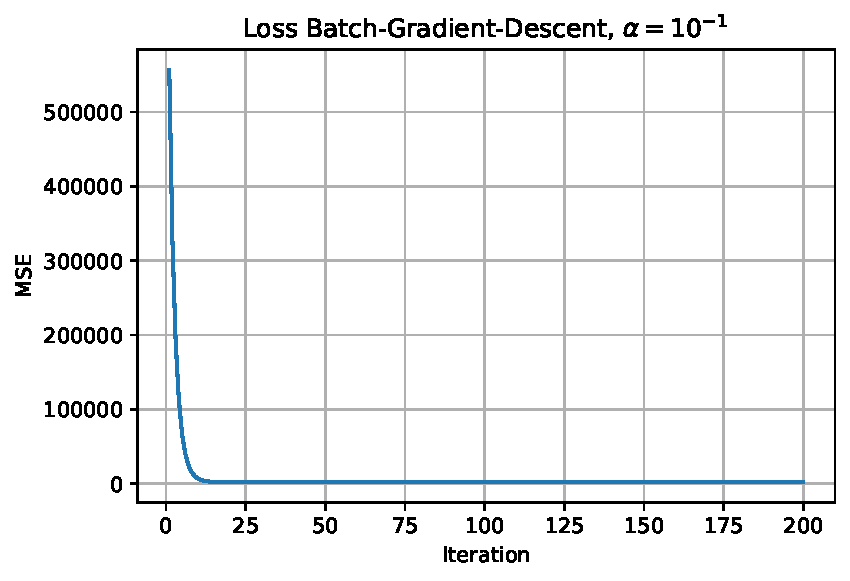
\includegraphics[width=0.5\linewidth]{figs/ex3_1_loss_bgd1.pdf}}
		\subfloat[Loss for SGD]{	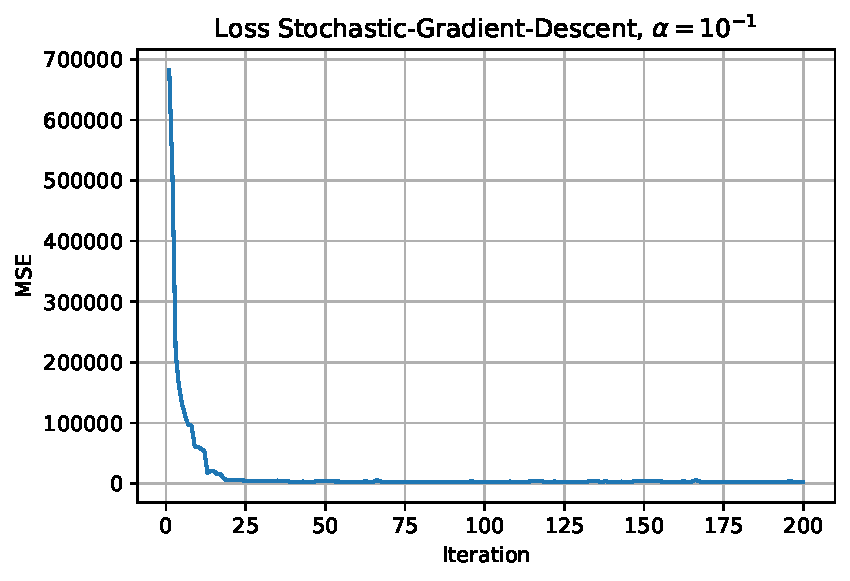
\includegraphics[width=0.5\linewidth]{figs/ex3_1_loss_sgd1.pdf}}

		\caption{Comparison BGD and SGD for higher learning rate}
		\label{fig:ex3_1_learning_rate}
	\end{figure}

	\subsection*{Epochs}
	One full iteration over the traing dataset is called an epoch.
	For BGD one iteration of the optimizer is one iteration over the training set, therefore $200$ epochs where performed in this example.
	
	For SGD one iteration uses only one sample, as the dataset includes $100$ samples, this means $2$ epochs where performed.
	
	For a large dataset I would choose SGD, because when using BGD the weights are only updated after going through all the training samples which would take up a lot of time. With SGD the weights are updated with each sample decreasing the computation time.
	
	
	\section*{Problem 3.2}
	
	\subsection*{XOR Approximation}
	
	The configuration in \prettyref{tab:ex3_2_xor} was found by selecting a linear activation function for the neuron in Layer 1. For both neurons in Layer 0 a relu activation function was choosen and the intermediate outputs $z_0^{(0)}$ and $z_1^{(0)}$ were selected as shown in the table.
	
	From there on the weights and biases can be found to give the desired outputs
	\begin{align}
		\matr{w}_0^{(0)} &= [-1, +2]  \quad b_0^{(0)}=-1 \quad \sigma_0^{(0)} = \mathrm{relu} \\
		\matr{w}_1^{(0)} &= [+2, -1]  \quad b_1^{(0)}=-1 \quad \sigma_1^{(0)} = \mathrm{relu} \\
		\matr{w}_0^{(1)} &= [+1, +1]  \quad b_0^{(1)}=0 \qquad \sigma_0^{(1)} = \mathrm{linear}
	\end{align}

	\begin{table}[H]
		\centering
		\begin{tabular}{r|r|r|r|r|r|r|r}
			$\matr{x}^T$     & $y$ & $a_0^{(0)}$ & $z_0^{(0)}$ & $a_1^{(0)}$ & $z_1^{(0)}$ & $a_0^{(1)}$ & $\hat{y}=z_0^{(1)}$ \\ \hline
			$[0,0]$ & $0$ & $-1$        & 0         &   -1     & 0         & 0         & 0                 \\ \hline
			$[0,1]$ & $1$ & $1$         & 1         &   -2     & 0         & 1         & 1                 \\ \hline
			$[1,0]$ & $1$ & $-2$        & 0         &   1     & 1         & 1         & 1                 \\ \hline
			$[1,1]$ & $0$ & $0$         & 0         &   0     & 0         & 0         & 0                
		\end{tabular}
		\caption{Network output and activations to approximate a logical XOR}
		\label{tab:ex3_2_xor}
	\end{table}
	
	\subsection*{Backpropagation}
	
	The loss function is $J\left(\matr{w}, b\right)= \left(y-\hat{y}\right)^2$. 
	The gradient with respect to the weights and bias of the first layer are
	\begin{align}
		\frac{\partial J}{\partial \matr{w}_0^{(1)}} &= \frac{\partial J}{\partial z_0^{(1)}} \frac{\partial z_0^{(1)}}{\partial a_0^{(1)}} \frac{\partial a_0^{(1)}}{\partial \matr{w}_0^{(1)}} \\
		\frac{\partial J}{\partial {b}_0^{(1)}} &= \frac{\partial J}{\partial z_0^{(1)}} \frac{\partial z_0^{(1)}}{\partial a_0^{(1)}} \frac{\partial a_0^{(1)}}{\partial {b}_0^{(1)}} 
	\end{align}

	As $\hat{y} = z_0^{(1)}$, $z_j^{(i)} = \sigma_j^{(i)}\left(a_j^{(i)}\right)$ and $a_j^{(i)} = \matr{w}_j^{(i)} \matr{z}^{(i-1)} + b_j^{(i)}$ the terms can be calculated to
	
	\begin{align}
		\frac{\partial J}{\partial z_0^{(1)}} &= 2\left(\hat{y}- y\right) \\
		\frac{\partial z_0^{(1)}}{\partial a_0^{(1)}} &= \frac{\partial \sigma_0^{(1)}\left(a_0^{(1)}\right)}{\partial a_0^{(1)}} = 1 \label{eq:nonlinearity} \\
		\frac{\partial a_0^{(1)}}{\partial \matr{w}_0^{(1)}} &= \left(\matr{z}^{(0)}\right)^T \\
		\frac{\partial a_0^{(1)}}{\partial {b}_0^{(1)}}  &= 1
	\end{align}
	
	where in \prettyref{eq:nonlinearity} a linear activation function was assumed, this term would change for a nonlinear activation function.
	Therefore, the gradients for layer 1 are
	\begin{align}
		\frac{\partial J}{\partial \matr{w}_0^{(1)}} &= 2\left(\hat{y}- y\right) \left(\matr{z}^{(0)}\right)^T \\
		\frac{\partial J}{\partial {b}_0^{(1)}} &= 2\left(\hat{y}- y\right).
	\end{align}
	
	Analogously the gradients for neuron $0$ of layer 0 are
	\begin{align}
		\frac{\partial J}{\partial \matr{w}_0^{(0)}} &= \frac{\partial J}{\partial z_0^{(1)}}\frac{\partial z_0^{(1)}}{\partial a_0^{(1)}} \frac{\partial a_0^{(1)}}{\partial z_0^{(0)}} \frac{\partial z_0^{(0)}}{\partial a_0^{(0)}}\frac{\partial a_0^{(0)}}{\partial \matr{w}_0^{(0)}} = 2\left(\hat{y}- y\right) w_{0,0}^{(0)} \matr{x}^T \\
		\frac{\partial J}{\partial {b}_0^{(0)}} &= \frac{\partial J}{\partial z_0^{(1)}}\frac{\partial z_0^{(1)}}{\partial a_0^{(1)}} \frac{\partial a_0^{(1)}}{\partial z_0^{(0)}} \frac{\partial z_0^{(0)}}{\partial a_0^{(0)}}\frac{\partial a_0^{(0)}}{\partial {b}_0^{(0)}} =2\left(\hat{y}- y\right) w_{0,0}^{(0)}
	\end{align}
	
	During optimization the gradient flows backwards through the network.
	First the gradient of the loss function with respect to the output of the last neuron is calculated 
	\begin{equation}
		\frac{\partial J}{\partial z_0^{(i)}}.
	\end{equation}
	
	With the weights, biases and activation function of the neuron the gradient with respect to the input of that neuron can be calculated
	\begin{equation}
		\frac{\partial z_0^{(i)}}{\partial z_0^{(i-1)}}
	\end{equation}
	which is then again passed backwards the the previous layer where this step is repeated until the input of the network is reached.
	
	In this way the calculation of the gradients with respect to all trainable variables can be calculated efficiently, because redundant calculations are avoided. The gradient information from the preceding layer is used to compute the gradient of the current layer.
	
	\subsection*{AND Approximation}
	
	A network with a linear activations in the first layer and a sigmoid in the second layer was trained to approximate a logical AND function. The network outputs are shown in \prettyref{tab:ex3_2_and}.
		The weights and biases are summarized in  \prettyref{eq:ex3_2_and1} to \prettyref{eq:ex3_2_and2}.
	
	\begin{table}[H]
		\centering
		\begin{tabular}{r|r|r|r|r|r|r|r}
			$\matr{x}^T$     & $y$ & $a_0^{(0)}$ & $z_0^{(0)}$ & $a_1^{(0)}$ & $z_1^{(0)}$ & $a_0^{(1)}$ & $\hat{y}=z_0^{(1)}$ \\ \hline
			$[0,0]$ & $0$ & \num{-3.6}       & \num{-3.6}         &  \num{-2.1}   & \num{-2.1}         & \num{-19}         & \num{4.2e-9}                 \\ \hline
			$[0,1]$ & $0$ & \num{-0.9}         & \num{-0.9}          &  \num{-0.6}    &  \num{-0.6}         & \num{-6.5}         & \num{1.5e-3}                 \\ \hline
			$[1,0]$ & $0$ & \num{-0.9}        & \num{-0.9}          &   \num{-0.5}    & \num{-0.5}         & \num{-6.5}         & \num{1.4e-3}                 \\ \hline
			$[1,1]$ & $1$ & \num{1.7}         & \num{1.7}         &   \num{1.0}     & \num{1.0}        & \num{6.2}         & \num{1.0}         
		\end{tabular}
		\caption{Network output and activations to approximate a logical AND}
		\label{tab:ex3_2_and}
	\end{table}
	
	\begin{align}
		\matr{w}_0^{(0)} &= [\num{2.6}, \num{2.7}] \quad b_0^{(0)}=\num{-3.6} \quad \sigma_0^{(0)} = \mathrm{linear} \label{eq:ex3_2_and1}\\
		\matr{w}_1^{(0)} &= [\num{1.6}, \num{1.5}]  \quad b_1^{(0)}=\num{-2.1} \quad \sigma_1^{(0)} = \mathrm{linear} \\
		\matr{w}_0^{(1)} &= [\num{3.6}, \num{2.1}]  \quad b_0^{(1)}=\num{-2.1} \quad \sigma_0^{(1)} = \mathrm{sigmoid} \label{eq:ex3_2_and2}
	\end{align}
	
	\section*{Problem 3.3}
	
	\subsection*{Number of trainable parameters}
	
	The summary of the baseline model can be seen below. For a dense layer with input size $n$ and output size of $m$ the number of parameters can be calculated by first considering the interconnections basically acting like a matrix of size $m\cross n$. Additionally there are $m$ bias terms adding up to a total number of $(n+1)m$ parameters.
	For \texttt{Layer1} this means $11\cdot128 = 1408$ parameters, because the input size is $10$.  For the \texttt{Output} layer it can be calculated by $129\cdot3 = 387$.
	
	\begin{lstlisting}[caption=Summary of baseline model]
_________________________________________________________________
Layer (type)                 Output Shape              Param #   
=================================================================
Layer1 (Dense)               (None, 128)               1408      
_________________________________________________________________
Layer2 (Dense)               (None, 128)               16512     
_________________________________________________________________
Layer3 (Dense)               (None, 128)               16512     
_________________________________________________________________
Output (Dense)               (None, 3)                 387       
=================================================================
Total params: 34,819
Trainable params: 34,819
Non-trainable params: 0
_________________________________________________________________
	\end{lstlisting}
	
The summary of the dropout model below shows that the dropout has exactly the same number of total parameters. The added dropout layers have no parameters, a certain percentage  of the connections is just dropped at random during training.
	
	
		\begin{lstlisting}[caption=Summary of dropout model]
_________________________________________________________________
Layer (type)                 Output Shape              Param #   
=================================================================
Layer1 (Dense)               (None, 128)               1408      
_________________________________________________________________
Drop1 (Dropout)              (None, 128)               0         
_________________________________________________________________
Layer2 (Dense)               (None, 128)               16512     
_________________________________________________________________
Drop2 (Dropout)              (None, 128)               0         
_________________________________________________________________
Layer3 (Dense)               (None, 128)               16512     
_________________________________________________________________
Drop3 (Dropout)              (None, 128)               0         
_________________________________________________________________
Output (Dense)               (None, 3)                 387       
=================================================================
Total params: 34,819
Trainable params: 34,819
Non-trainable params: 0
_________________________________________________________________
	\end{lstlisting}
	
	\subsection*{Comparison of the models}
	
	In \prettyref{fig:ex3_3_learning_curves} the learning curves for both models on both datasets are shown.
	
  On the train dataset the baseline model can decrease the loss further achieving a better accuracy than the dropout model. The loss of the dropout model stays relatively constant from epoch $50$ on.
  On the test set it can be seen that the baseline model is already in an overfitting regime from iteration $25$ on, because the loss on the test set increases again and the accuracy gets worse.
  The dropout model does not suffer from this effect, its performance stays constant from epoch $50$ on.
	
	The final accuracy for the baseline model was \SI{89.5}{\percent}, for the dropout model it was \SI{92.3}{\percent} on the test set.

	\begin{figure}[H]
	\centering	
	\subfloat[Train dataset]{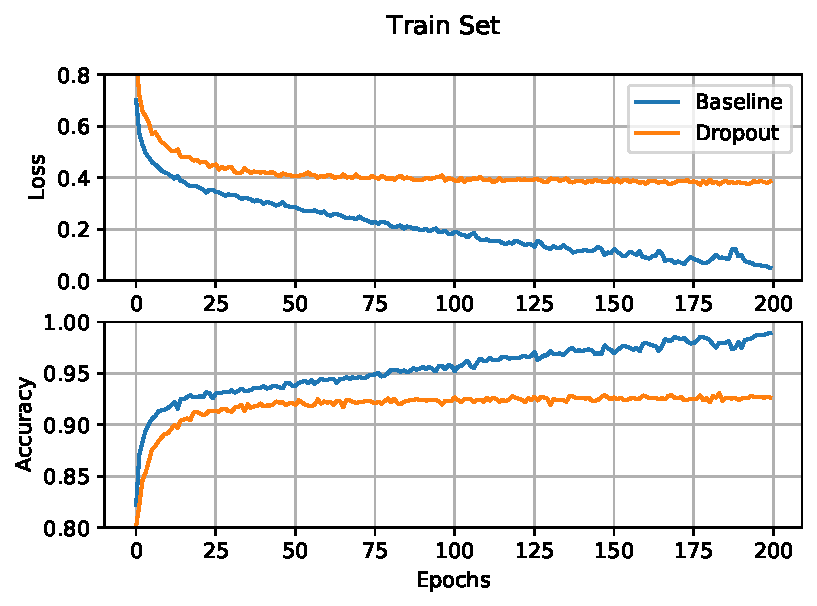
\includegraphics[width=0.5\linewidth]{figs/ex3_3_train.pdf}}
	\subfloat[Test dataset]{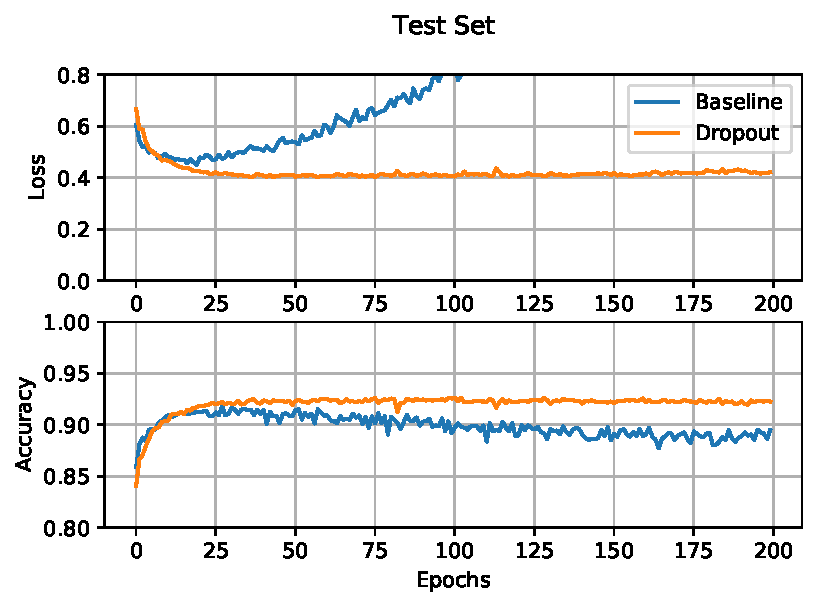
\includegraphics[width=0.5\linewidth]{figs/ex3_3_test.pdf}}
	\caption{Learning curves on the two datasets for both models}
	\label{fig:ex3_3_learning_curves}
	\end{figure}

	\subsection*{Early Stopping}
	
	Another approach to regularization and avoiding overfitting is early stopping. The corresponding plots are shown in \prettyref{fig:ex3_3_learning_curves_early}. The training process is stopped earlier, when for a certain number of epochs the loss decreases less than a specified amount.
	The training process is stopped after iteration $25$. As can be seen this is before the loss on the test set starts increasing.
	
		The final accuracy for the baseline model was \SI{90.8}{\percent}, for the dropout model it was \SI{92.3}{\percent} on the test set. The baseline model thus performs better with early stopping than when optimizing for the whole $200$ epochs, because overfitting is avoided.
	
	
		\begin{figure}[H]
		\centering	
		\subfloat[Train dataset]{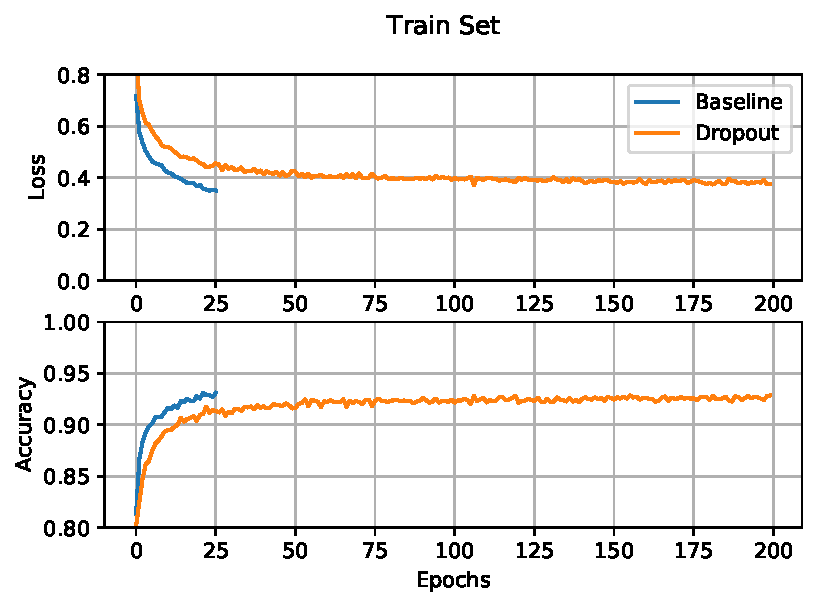
\includegraphics[width=0.5\linewidth]{figs/ex3_3_train_early.pdf}}
		\subfloat[Test dataset]{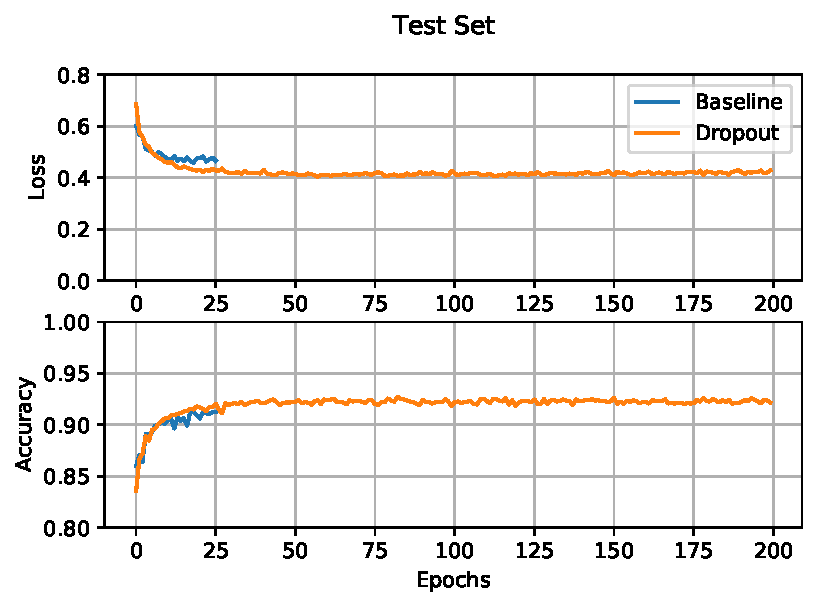
\includegraphics[width=0.5\linewidth]{figs/ex3_3_test_early.pdf}}
		\caption{Learning curves on the two datasets for both models}
		\label{fig:ex3_3_learning_curves_early}
	\end{figure}

	\subsection*{Housing dataset}
	
	A neural network was then used to perform regression on the housing dataset. As the loss the mean absolute error (MAE) was choosen. The network structure is summarized below. 
	A graph is shown in \prettyref{fig:ex3_3_nngraph}. For the hidden layers a relu activation function has been selected. For the output layer a linear layer was selected.
	For the dropout layers a rate of $0.15$ was selected. The batch size was set to $64$. 
	The learning curve is shown in \prettyref{fig:ex3_3_learning_curve_housing}.
	The final MAE on the test set was \num{0.312}.
	In the shown number of epochs the loss on both datasets decreases, indicating that the model is not yet overfitting.
	
	
\begin{lstlisting}[caption=Neural network for the housing dataset]
_________________________________________________________________
Layer (type)                 Output Shape              Param #   
=================================================================
Layer1 (Dense)               (None, 128)               1152      
_________________________________________________________________
Drop1 (Dropout)              (None, 128)               0         
_________________________________________________________________
Layer2 (Dense)               (None, 128)               16512     
_________________________________________________________________
Drop2 (Dropout)              (None, 128)               0         
_________________________________________________________________
Layer3 (Dense)               (None, 64)                8256      
_________________________________________________________________
Drop3 (Dropout)              (None, 64)                0         
_________________________________________________________________
Output (Dense)               (None, 1)                 65        
=================================================================
Total params: 25,985
Trainable params: 25,985
Non-trainable params: 0
_________________________________________________________________
\end{lstlisting}

	\begin{figure}[H]
		\centering	
		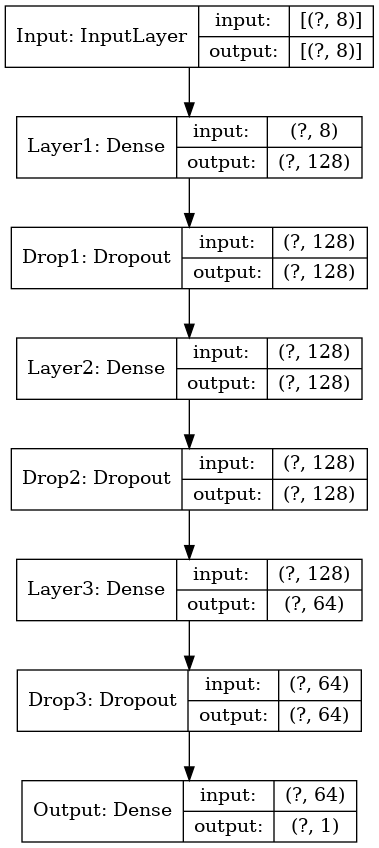
\includegraphics[width=0.3\linewidth]{figs/ex3_3_model}
		\caption{Graphical representation of the network}
		\label{fig:ex3_3_nngraph}
	\end{figure}

	\begin{figure}[H]
		\centering	
		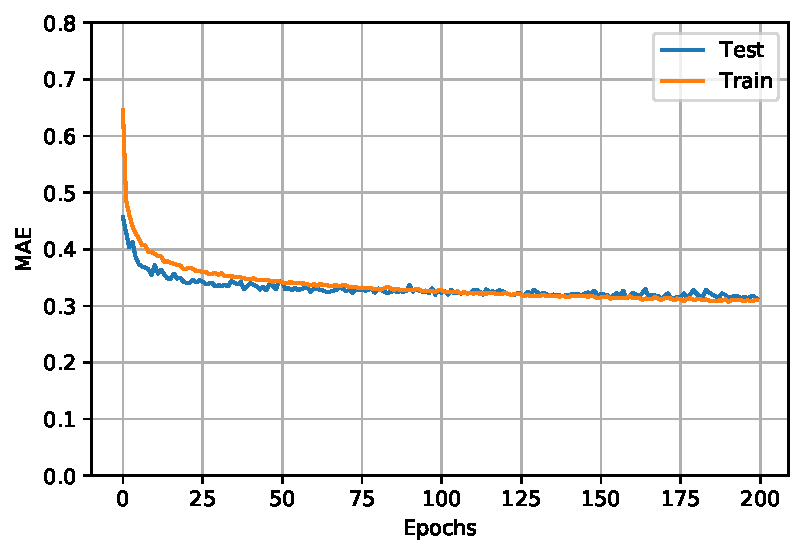
\includegraphics[width=0.5\linewidth]{figs/ex3_3_housing_learning_curve}
		\caption{Learning curve for the network on the housing dataset}
		\label{fig:ex3_3_learning_curve_housing}
	\end{figure}

\end{document}